\documentclass[fleqn,10pt]{wlscirep}
\usepackage[utf8]{inputenc}
\usepackage[T1]{fontenc}
\usepackage{textcomp}
\title{Tropopause}

% \author[1]{Peter Phan}
% \author[2, 3]{Hamed Ibrahim}
% % \author[1,2,+]{Christine Author}
% % \author[2,+]{Derek Author}
% \affil[1]{University of Toronto, Department of Mechanical and Industrial Engineering}
% \affil[2]{University of Toronto, Department of Civil and Mineral Engineering}
% \affil[3]{University of Toronto, School of the Environment}

% \affil[1]{tammy.phan@utoronto.ca}

%\affil[+]{these authors contributed equally to this work}

%\keywords{Keyword1, Keyword2, Keyword3}

\begin{abstract}
Example Abstract. Abstract must not include subheadings or citations. Example Abstract. Abstract must not include subheadings or citations. Example Abstract. Abstract must not include subheadings or citations. Example Abstract. Abstract must not include subheadings or citations. Example Abstract. Abstract must not include subheadings or citations. Example Abstract. Abstract must not include subheadings or citations. Example Abstract. Abstract must not include subheadings or citations. Example Abstract. Abstract must not include subheadings or citations.
\end{abstract}
\begin{document}

\flushbottom
\maketitle
% * <john.hammersley@gmail.com> 2015-02-09T12:07:31.197Z:
%
%  Click the title above to edit the author information and abstract
%
\thispagestyle{empty}

%\noindent Please note: Abbreviations should be introduced at the first mention in the main text – no abbreviations lists. Suggested structure of main text (not enforced) is provided below.

\section{Introduction}
\cite{meng2021continuous}

The tropopause is the atmospheric boundary that separates the troposphere and stratosphere, and is defined by stark differences in both thermal structure and chemical composition of the two atmospheric layers. The tropopause is sensitive to climate variability and may thus serve as one of many indicators of the effects of climate change. The height of the tropopause has been increasing in the past few decades, a trend detected in a number of diverse data sources including radiosonde observations, reanalysis data, and climate model simulations. This rise is closely associated with tropospheric warming and stratospheric cooling \cite{santer2003contributions},\cite{seidel2006variability}. Additionally, it has been suggested that the tropopause is itself an atmospheric layer rather than a sharp demarcation \cite{feng2012trends}. Taking this perspective, the vertical extent of the tropopause layer has also been found to be increasing, correlated with decreasing temperature of the layer's top i.e., the lower stratosphere \cite{feng2012trends}. A number of studies on tropopause characteristics have been completed through analyzing a variety of rich data sources. Meng et al. used comprehensive radiosonde data, as well as satellite GPS radio occultation (RO) measurements to assess the change in tropopause height due to temperature variations in the troposphere and stratosphere, changes in anthropogenic activities, GHG emissions and stratospheric ozone changes. Their analysis also considered major natural forcings, and even after removing this variability, it is concluded that there has been a continuous rise of the tropopause in the Northern Hemisphere (NH) after the year 2000 due to tropospheric warming. Feng et al. \cite{feng2012trends} characterized the tropopause as an atmospheric layer and analyzed radiosonde data between 1965-2004. They concluded the thickness of this tropopause layer has been increasing during this time period, along with an increase in its altitude and a cooling of the layer's top. In this paper, we present the most comprehensive and up-to-date analysis of the tropopause. We examine trends in its height, thickness, pressure, temperature, its response to natural and anthropogenic forcings, as well as its alternative definitions and characterizations. We consider a comprehensive number of sources including reanalysis data, radiosonde data, and GPS data. 














\section{Methods}
\subsection*{Time periods}
Following Xian and Homeyer\cite{xian2019global} and Meng et al.\cite{meng2021continuous}, we use the IGRA2 dataset. We take only data recorded at 0000 UTC and 1200 UTC, but treat records from 2100 to 0300 UTC as 0000 UTC and from 0900 to 1500 UTC as 1200 UTC. We conduct analyses over three time periods: the first from 1980 to 2020, the second from 2000 to 2024, and the third from 2015 to 2024. For each analysis, we hand select stations based on their data availability and data quality. Both the first and second tropopause are calculated using the WMO lapse-rate definition. 
\subsection*{Methods to compute the tropopause}
There are multiple ways to compute the tropopause from gridded data. We compare two methods: the pressure-level based method of Reichler et al. \cite{reichler2003determining}, and the model-level or altitude-based method of Zangl and Hoinka \cite{zangl2001tropopause}. Additionally, we may compute the tropopause in terms of either geopotential or geometric height. In reality, the geopotential and geometric height at the altitude the tropopause is at only differ by tens of meters. Nonetheless, we will compute both. 
\subsubsection*{Interpolation}
It is important to note that the variables will vary depending on the interpolation method used as well as the interpolation resolution. \textbf{Test both}.








\subsection{IGRA \cite{durre2006overview}} 
\subsection*{Global tropopause altitudes in radiosondes and reanalyses, Xian and Homeyer\cite{xian2019global}}
Launches that occured between 2100 and 0300 UTC were included with 0000 UTC. Launches between 0900 and 1500 UTC were included with 1200 UTC. Radiosonde data is linearly interpolated to a 200m resolution prior to tropopause identification. Only sounds with observations within 5-22km are included. Both the first and second tropopause (if present) are identified according to the WMO lapse-rate definition. Lapse rates are calculated with finite differences i.e., $-\partial T/\partial z \approx -(T_{i+1} - T_i)/(z_{i+1} - z_i)$. Trends over the period 1981-2015 are studied using monthly mean first tropopause altitudes and monthly fraction of profiles with double tropopauses. Monthly mean or double tropopause fraction is computed only when a station has $\geq 20$ days of valid data i.e., from either 0000 and 12000 and all levels up to 22km. Trends are calculated for stations that have valid data for at least half of the total number of months in the 35-year period and a roughly even distribution of data throughout the period i.e., data gaps must be less than 5 years and there is no missing data near the beginning/end of the time series. Monthly tropopause time series are deseasonalized with a high-pass filter, removing variability at timescales $\leq 1$ year. Linear regression on the filtered time series is used to measure trends over the 35 years. Trends are deemed significant if they exceed the 3$\sigma$ uncertainty of the measured slope, which is analogous to statistical significance at the 99\% confidence level for a
Gaussian distribution.


\subsection*{Variability and trends in the global tropopause estimated from radiosonde data, Seidel and Randel\cite{seidel2006variability}}
Radiosonde data from 1958-2004 from 100 stations were taken from the IGRA \cite{durre2006overview}, depending on the length and completesness of the record. Stations were selected with the goal of global coverage. All soundings within three hours of 0000 or 1200 UTC were taken. Data on pressure, temperature and geopotential height were taken. Height was interpolated when necessary. The LRT data in the sounding data was ignored, and the first and second tropopause (if present) were calculated using the WMO lapse rate definition. Temperature and height at the surface and at 850, 500, 300, 200, 150, 100, 70, 50, 30, 20 hPa. The layer mean temperature for 850-300 and 100-50 hPa were calculated. Soundings with no LRT or suspicious data were excluded. Time series for analysis of variability on four timescales (synoptic, monthly, seasonal, multidecadal) were separately made for each time (0000 and 1200). 

Mean seasonal cycle was calculated by averaging all soundings for each calendar month. Monthly means for each month were calculated if $\geq 50\%$ of the observations were available. Monthly anomaly time series were computed by subtracting the mean seasonal cycle from the monthly means, and these anomalies were used in estimating multidecadal trends. Synoptic variations were defined as the departure of daily values from the monthly mean for the relevant month and year.

Radiosonde measurements suffer from temporal homogeneity \cite{gaffen1994temporal, parker1995towards, seidel2001climatological, redder2004unexplained, lanzante2003temporal, sherwood2005radiosonde, randel2006biases}. The homogeneity adjustments in the data sets of Free\cite{free2005radiosonde}, Thorne\cite{thorne2005revisiting} are not suitable for tropopause study, because the adjusted data are monthly anomaly time series. Thus, stations with inhomogeneous data were excluded, as well as stations with more than one third of the monthly anomalies missing. 

\subsection*{Trends in the global tropopause thickness revealed by radiosondes, Feng et al. \cite{feng2012trends}}
Following Feng et al. \cite{feng2012trends}. Data was taken from 187 stations from 1965 to 2004. Only soundings up to 70 hPa were considered. Both first and second tropopause height was calculated from the WMO lapse-rate definition with the algorithm in Reichler et al. \cite{reichler2003determining}. The thickness of the tropopause layer is the difference between the second and first tropopause. If a first tropopause is detected above 40 hPa or below 500 hPa, it was removed. For each month, we calculate the average of all available soundings. Trend analysis was done by subtracting monthly mean over 1965 to 2004 from the individual monthly mean, to give monthly anomalies. To calculate trend uncertainties, a 95\% confidence interval was calculated with a $t$ test. For example, if the trend in temperature increase is 0.2\textdegree C per decade with a 95\% confidence interval of $\pm$0.05\textdegree C, the true trend is likely between 0.15\textdegree C and 0.25\textdegree C per decade.
\subsection*{Continuous rise of the tropopause in the Northern Hemisphere over 1980–2020, Meng et al. \cite{meng2021continuous}}
Meng et al. \cite{meng2021continuous} used data from 149 hand-selected stations from the IGRA2 dataset. Stations were selected based on the length and completeness of their sounding records over 1980-2020. Tropopause height was calculated via the WMO lapse-rate definition. The method from Zangl and Hoinka \cite{zangl2001tropopause} was used to determine the height from the geopotential height and temperature profiles in each station record. Since each station differs in vertical resolution, the records were first linearly interpolated to a 200-m resolution before tropopause identification. The height was considered valid if it was between 5-18 km, The records extend at least 2km above the height, and the height is within 2 standard deviations of the 1980-2020 mean \textit{at that station}. Daily mean height was calculated if data was available at both 0000 and 1200 UT. If not, records between 2100-0300 were treated as 0000 UT and 0900-1500 UT as 1200 UT. The monthly mean was calculated for a given month if the daily means of $H$ were available for at least 15 days. If more than 30\% of stations have no monthly mean for a given month, we treat the month as missing data. Trend analysis was done by producing a time series of the monthly deviation of $H$ i.e., given a single month and year and its mean, subtract the whole time-span monthly mean from this to measure the anomaly. Using the same procedure, daily mean, monthly mean and monthly anomalies at the pressure levels $925, 850, 700, 500, 400, 300, 250, 200, 150, 100, 70, 50, 30, 20$ and surface pressure were calculated. Tropospheric temperature is the mean of temperature at 850,700,500,400,300 and lower stratospheric temperature is the mean of temperature at 100 and 70. If a value is missing at just one of these pressure levels, we ignore that month entirely and treat it as missing data. 

The selected stations must satisfy (1) the end year of the records is later than 2016 inclusive and the total number of soundings is $\geq 10,000$. (2) In $\geq 80\%$ of the years, there exist valid annual means of all the studied variables: $H$, temperature at 850, 700, 500, 400, 300, 250, 200, 150, 100, and 70 hPa, layer mean temperature over each of the two subperiods. An annual mean is valid iff the monthly means exist for $\geq 8$ months and every season contains at least one monthly mean in that year. 

\subsection*{Temperature and tropopause characteristics from reanalyses data in the tropical tropopause layer \cite{tegtmeier2020temperature}}

Raw radiosonde datasets e.g., the IGRA suffer from inhomogeneities and biases due to changes in instruments and measurement techniques. In this study, corrected radiosonde datasets are used instead of the IGRA, namely RATPAC \cite{free2005radiosonde}, RAOBCORE \cite{haimberger2007homogenization}, RICH \cite{haimberger2012homogenization}, and HadAT \cite{thorne2005revisiting} at 70 and 100 hPa. Interannual anomalies of cold point temperature, height, and pressure are done on the IGRA data itself because temperature corrections can change the location of the cold point. Cold-point temperature trend are analyzed via adjusted cold point trends from the corrected data. 

\subsection{Radio Occultation Measurements}
\subsection*{Temperature and tropopause characteristics from reanalyses data in the tropical tropopause layer \cite{tegtmeier2020temperature}}
Temperature and pressure data are also available via the GNSS-RO technique. A monthly mean zonal mean dataset is constructed from measurements collected by various missions \cite{wickert2001atmosphere, beyerle2005gps, anthes2008cosmic, von2011gras, hajj2004champ, beyerle2011first}. The observational temperature records at reanalysis model levels are computed by interpolating each GNSS-RO profile to the reanalysis model levels with the barometric formula. The WMO lapse rate and cold point definitions are used. Daily data of cold point temperatures from all GNSS-RO missions between 30\textdegree N and  30\textdegree S. 

To detect Kelvin wave anomalies for planetary wavenumbers 1-15, periods 4-30 d and equivalent depths of 6-600, a 2D FFT is applied to each 5\textdegree wide latitude band \cite{wheeler1999convectively}. The filtered anomalies represent cold point temperature variability that propagates in the same wavenumber–frequency domain as Kelvin waves, i.e., when the temperature is modulated by Kelvin waves present around the tropopause. To measure the amount of Kelvin wave activity in the TTL, the spatial variance of the filtered signals is used to calculate a monthly index. The index is the $1\sigma$ standard deviation over the filtered anomalies at all spatial grid points. Time periods
of enhanced Kelvin wave activity are defined as the months when the index is larger than the long-term mean plus the $1\sigma$ standard deviation of the whole time series.

\subsection{Station criteria}
\subsection*{Global tropopause altitudes in radiosondes and reanalyses, Xian and Homeyer\cite{xian2019global}}
Station must have at least 20 days of suitable profiles to compute a monthly mean. A suitable profile has measurements at all mandatory and significant levels up to 22km or higher, all at either 0000 or 1200 UTC. Long-term trends are calculated for stations that meet this criteria for at least half the months from 1981 to 2015 and a roughly even distribution of data throughout the period i.e., any gaps must be less than 5 years and there must be no missing data near the beginning or the end of the period. 
\subsection*{Variability and trends in the global tropopause estimated from radiosonde data, Seidel and Randel\cite{seidel2006variability}}
Stations were selected on the basis of the length and completeness of their data and an aim for global coverage. Complete station ID list: ['ARM00087576', 'ASM00094120', 'ASM00094294', 'ASM00094610', 'ASM00094672', 'ASM00094998', 'AYM00089009', 'AYM00089050', 'AYM00089532', 'AYM00089542', 'AYM00089564', 'AYM00089664', 'BDM00078016', 'BPM00091517', 'BRM00082332', 'BRM00083746', 'CAM00071072', 'CAM00071082', 'CAM00071801', 'CAM00071836', 'CAM00071926', 'CHM00051709', 'CHM00052681', 'CIM00085442', 'CIM00085469', 'CIM00085799', 'COM00080222', 'FIM00002836', 'FJM00091680', 'FMM00091334', 'FPM00091938', 'FSM00061996', 'GIM00008495', 'GLM00004360', 'GMM00010868', 'HKM00045004', 'ICM00004018', 'IOM00061967', 'ISM00040179', 'IVM00065578', 'JAM00047401', 'JAM00047827', 'JAM00047991', 'JNM00001001', 'KEM00063741', 'LYM00062010', 'MAM00067083', 'NFM00094996', 'NGM00061052', 'NZM00093844', 'NZM00093986', 'POM00008508', 'PSM00091408', 'RMM00091376', 'RQM00078526', 'RSM00021504', 'RSM00021965', 'RSM00023415', 'RSM00023472', 'RSM00024266', 'RSM00028698', 'RSM00030230', 'RSM00032540', 'RSM00034731', 'RSM00035121', 'SAM00041024', 'SFM00068588', 'SFM00068816', 'SFM00068994', 'SGM00061641', 'SHM00061902', 'SHM00068906', 'SNM00048698', 'SPM00060020', 'THM00048455', 'TXM00038880', 'UKM00003005', 'USM00070026', 'USM00070273', 'USM00070308', 'USM00070398', 'USM00072201', 'USM00072208', 'USM00072250', 'USM00072251', 'USM00072293', 'USM00072327', 'USM00072403', 'USM00072451', 'USM00072493', 'USM00072520', 'USM00072645', 'USM00072694', 'USM00072712', 'USM00072747', 'USM00072768', 'USM00072776', 'USM00072797', 'USM00091165', 'USM00091285']. 
\subsection*{Trends in the global tropopause thickness revealed by radiosondes, Feng et al. \cite{feng2012trends}}
Used a pre-selected list of stations\cite{wallis1998subset}
\subsection*{Continuous rise of the tropopause in the Northern Hemisphere over 1980–2020, Meng et al. \cite{meng2021continuous}}
Each selected station must satisfy: the end year of stations is later than 2016 inclusive and the total number of soundings is over 10,000, the station has valid annual means of all the studied variables (tropopause height $H$, temperature at 850, 700, 500, 400, 300, 250, 200, 150, 100, and 70 hPa, and layer mean temperaturee of 850 to 300 and 100 to 70 hPa over both 1980-2000 and 2001-2020). An annual mean is valid if the monthly means are available in at least 8 months and every season contains at least one monthly mean. 

\newpage 
\section*{Appendix}
\subsection*{Reichler, Dameris, and Sausen method for computing the tropopause\cite{reichler2003determining}}
We use the WMO lapse rate definition: ``the lowest level at which the lapse-rate decreases to 2\textdegree C/km
or less, provided that the average lapse-rate between this level
and all higher levels within 2 km does not exceed 2\textdegree C/km''. Recall that the lapse-rate is defined as
\[\Gamma = -\frac{\partial T}{\partial z}\]
Suppose we have data of the form $\{(T_i, p_i)\}^{N}_{i=1}$ where $T$ is temperature and $p$ is pressure. We may then convert the lapse-rate equation to 
\[\Gamma = -\frac{\partial T}{\partial z} = -\frac{\partial T}{\partial p}\frac{\partial p}{\partial z} = -\frac{\partial T}{\partial p^\kappa}\frac{\partial p^\kappa}{\partial p}\frac{\partial p}{\partial z}\]
where $R$ is the dry air gas constant, $c_p$ is the specific heat capacity of air at constant pressure, and $\kappa = R/c_p$. Given the hydrostatic approximation, we may then convert this to 
\[\Gamma(p) = \frac{\partial T}{\partial p^\kappa}\frac{p^\kappa}{T}\left(\frac{\kappa g}{R}\right)\]
Define the pressure at the half levels as the mean of the pressures of the last and next level:
\[p^{\kappa}_{i+1/2} = \frac{p^\kappa_i + p^\kappa_{i+1}}{2}\]
Approximate the lapse-rate at the half-levels by finite differencing:
\[\Gamma_{i+1/2} = \frac{T_{i+1} - T}{p^\kappa_{i+1} - p^\kappa_{i}}\frac{p^\kappa_i + p^\kappa_{i+1}}{T_i + T_{i+1}}\left(\frac{\kappa g}{R}\right)\]
Then search for the lowest half-level $p_{j+1/2}$ where $\Gamma_{j+1/2} < 2 \textdegree C/km$. Then check if the mean lapse-rates of the 2km layer above $p_{j+1/2}$ is below $\Gamma_{j+1/2}$. If both are true, we define the tropopause pressure by linearly interpolating between the half levels $j-1/2$ and $j+1/2$,
\[p_{TP}^\kappa = p^\kappa_{j-1/2} + \frac{p^\kappa_{j+1/2} - p^\kappa_{j-1/2}}{\Gamma_{j+1/2} - \Gamma_{j-1/2}}(2 - \Gamma_{j-1/2})\]
The search space of the pressure levels is limited between 550 hPa and 75 hPa. If no tropopause is found, then the data is simply recorded as missing. These missing values can be linearly interpolated after all other values are found. 
\subsection*{Z\"{a}ngl and Hoinka method for computing the tropopause\cite{zangl2001tropopause}}
Let $z_{i}$ be the geometric height at a record level $i$, $T_i$ be the temperature at a record level $i$. We first define the temperature gradient at the level $z_{i+1/2} = (z_i + z_{i+1})/2$ as 
\[\left(\frac{\partial T}{\partial z}\right)_{i+1/2} = \frac{T_{i+1} - T_i}{z_{i+1} - z_i}\]
We then check for the lowest level $i$ that fulfills $-(\partial T/\partial z)_{i + 1/2} \leq 2$ and $-(\partial T/\partial z)_{i - 1/2} > 2$, and set 
\[z_{TP} = z_{i-1/2} + \frac{z_{i+1/2} - z_{i-1/2}}{(\partial T/\partial z)_{i+1/2} - (\partial T/\partial z)_{i-1/2}}(2 + (\partial T/\partial z)_{i+1/2})\]
We then check if $(T_i - T_{TP})/(z_i - z_{TP}) < 2$ for all $i$ where $0 < z_i - z_{TP} \leq 2$ km. The search starts at 2000m. If the lapse rate never exceeds 2\textdegree C/km for all levels, we set the tropopause to 3.5km. If the lapse rate exceeds 2\textdegree C/km for all levels, we set the tropopause to 90 hPa. 
\subsection*{Xian and Homeyer Method\cite{xian2019global}}
In Xian and Homeyer, the radiosonde data is first interpolated to a 200m grid. The lapse rate is calculated via an upwards finite difference $\Gamma(z_i) \approx (T_{i+1} - T_i)/(z_{i+1} - z_i)$. The tropopause is then checked for similar to the above methods, but only within 5-22km. Geopotential altitude is used, and only stations with sufficient data between 5-22km are considered. 


















\newpage 
\newpage 
% The Introduction section, of referenced text\cite{Figueredo:2009dg} expands on the background of the work (some overlap with the Abstract is acceptable). The introduction should not include subheadings.

\section*{Results}

Up to three levels of \textbf{subheading} are permitted. Subheadings should not be numbered.

\subsection*{Subsection}

Example text under a subsection. Bulleted lists may be used where appropriate, e.g.

\begin{itemize}
\item First item
\item Second item
\end{itemize}

\subsubsection*{Third-level section}
 
Topical subheadings are allowed.

\section*{Discussion}

The Discussion should be succinct and must not contain subheadings.

\section*{Methods}

Topical subheadings are allowed. Authors must ensure that their Methods section includes adequate experimental and characterization data necessary for others in the field to reproduce their work.

\bibliography{sample}

\noindent LaTeX formats citations and references automatically using the bibliography records in your .bib file, which you can edit via the project menu. Use the cite command for an inline citation, e.g.  \cite{Hao:gidmaps:2014}.

For data citations of datasets uploaded to e.g. \emph{figshare}, please use the \verb|howpublished| option in the bib entry to specify the platform and the link, as in the \verb|Hao:gidmaps:2014| example in the sample bibliography file.

\section*{Acknowledgements (not compulsory)}

Acknowledgements should be brief, and should not include thanks to anonymous referees and editors, or effusive comments. Grant or contribution numbers may be acknowledged.

\section*{Author contributions statement}

Must include all authors, identified by initials, for example:
A.A. conceived the experiment(s),  A.A. and B.A. conducted the experiment(s), C.A. and D.A. analysed the results.  All authors reviewed the manuscript. 

\section*{Additional information}

To include, in this order: \textbf{Accession codes} (where applicable); \textbf{Competing interests} (mandatory statement). 

The corresponding author is responsible for submitting a \href{http://www.nature.com/srep/policies/index.html#competing}{competing interests statement} on behalf of all authors of the paper. This statement must be included in the submitted article file.

\begin{figure}[ht]
\centering
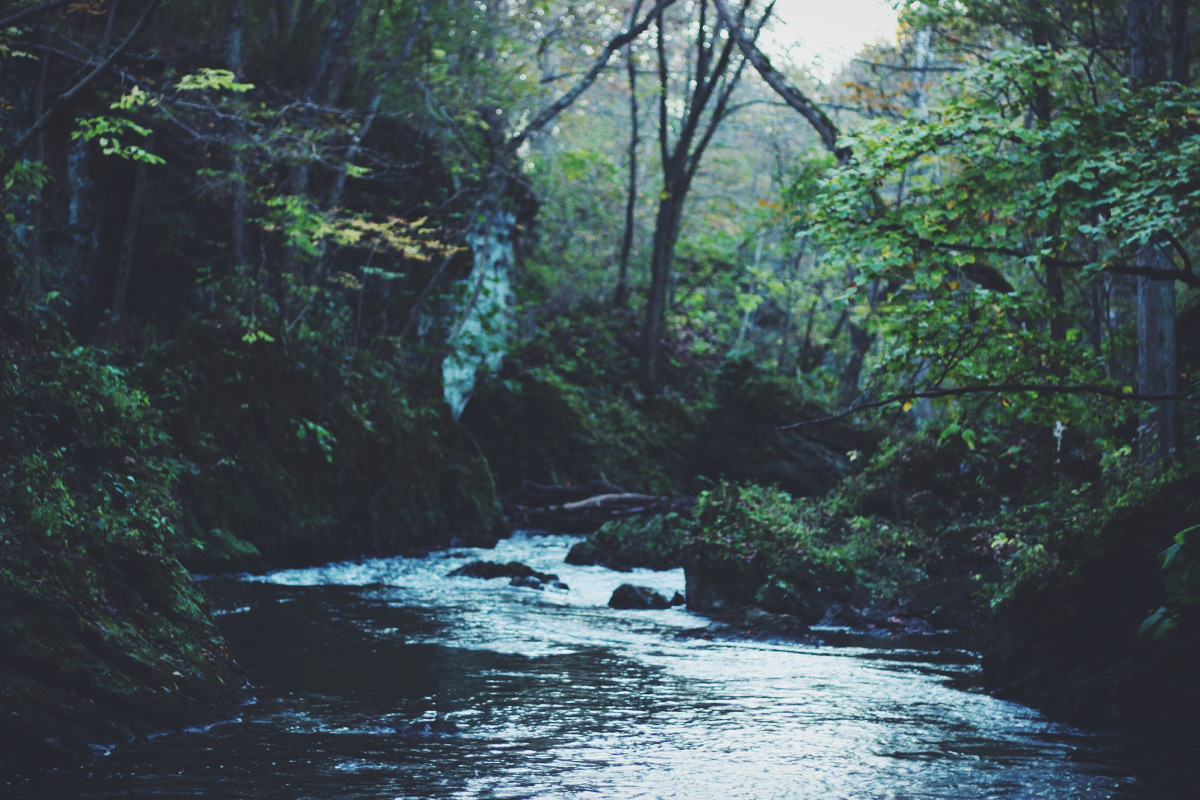
\includegraphics[width=\linewidth]{stream}
\caption{Legend (350 words max). Example legend text.}
\label{fig:stream}
\end{figure}

\begin{table}[ht]
\centering
\begin{tabular}{|l|l|l|}
\hline
Condition & n & p \\
\hline
A & 5 & 0.1 \\
\hline
B & 10 & 0.01 \\
\hline
\end{tabular}
\caption{\label{tab:example}Legend (350 words max). Example legend text.}
\end{table}

Figures and tables can be referenced in LaTeX using the ref command, e.g. Figure \ref{fig:stream} and Table \ref{tab:example}.

\end{document}